\subsection{Unraveling the Mystery of Roaring AC Line Noise!}

\begin{tcolorbox}[colback=gray!10, colframe=black, title=E4E10] Which of the following can create intermittent loud roaring or buzzing AC line interference? 
\begin{enumerate}[label=\Alph*),noitemsep]
    \item Arcing contacts in a thermostatically controlled device
    \item A defective doorbell or doorbell transformer inside a nearby residence
    \item A malfunctioning illuminated advertising display
    \item \textbf{All these choices are correct}
\end{enumerate} \end{tcolorbox}

\subsubsection{Concepts Related to AC Line Interference}

AC line interference can be a significant issue in electronic communication and other electrical systems. To understand the potential sources of this interference, we must consider various components and devices that might introduce noise into the AC power lines.

1. \textbf{Arcing contacts}: Devices that control temperature, such as thermostats, may utilize relays or contactors which, if they begin to wear out or fail, can create arcs. These arcs generate radio frequency interference (RFI) that manifests as loud buzzing or roaring sounds within the AC line.

2. \textbf{Defective doorbells or transformers}: Transformers that power doorbells can also malfunction over time and might generate noise due to electromagnetic interference (EMI). If the doorbell is close enough to the AC power lines, it can couple that interference back into the power lines.

3. \textbf{Malfunctioning illuminated displays}: High-intensity displays used in advertising often employ high voltage and current to operate their lighting. A failure in these displays can also produce AC line noise, contributing to the buzzing or roaring sounds experienced.

Each of these potential sources can independently contribute to line interference, and thus the correct answer, D, emphasizes that all listed options can generate such noise.

\subsubsection{Calculations and Diagrams}

While the question does not require specific calculations, understanding the impact of noise on AC circuits can involve some analysis. For instance, if we were to measure the interference on an AC line, we might use a spectrum analyzer to gain insights into both frequency and amplitude of the noise generated by the malfunctioning devices.

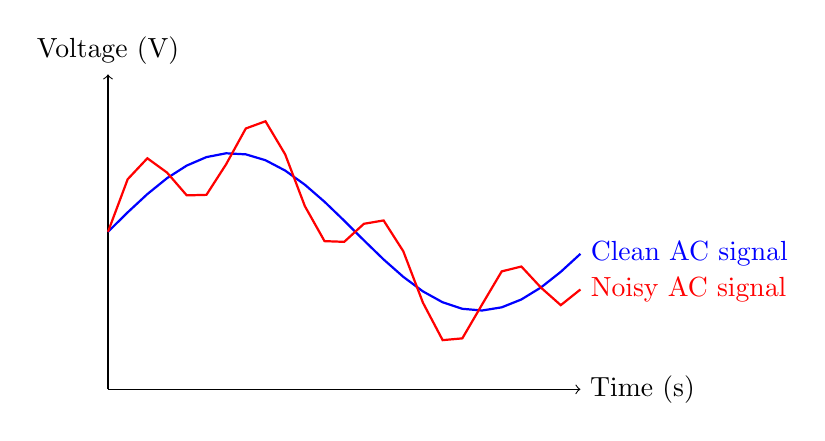
\begin{tikzpicture}
\draw[->] (0,0) -- (0,4) node[above]{Voltage (V)};
\draw[->] (0,0) -- (6,0) node[right]{Time (s)};
\draw[blue,thick] plot[domain=0:6] (\x, {2 + sin(\x r)}) node[right] {Clean AC signal};
\draw[red,thick] plot[domain=0:6] (\x, {2 + sin(\x r) + 0.5*sin(4*\x r)}) node[right] {Noisy AC signal};
\end{tikzpicture}

The diagram illustrates how a clean AC signal (blue) can be disrupted by noise (red), highlighting the signature of unwanted interference contributed by various sources, such as those listed in the question.
